\chapter{Model Comparison}
\label{ch:comparison}

This chapter presents a comparative analysis of the classification models — K-Nearest Neighbors (KNN) and Naïve Bayes — across the Raisin and HTRU2 datasets. Evaluation is based on accuracy, confusion matrices, and feature scalability.

\section{Accuracy Comparison}
\label{sec:comp_accuracy}

Table~\ref{tab:comp_accuracy} highlights the maximum accuracy obtained by both models on each dataset.

\begin{table}[H]
    \centering
    \caption{Maximum Accuracy Comparison of KNN vs Naïve Bayes}
    \label{tab:comp_accuracy}
    \begin{tabular}{|c|c|c|}
        \hline
        \textbf{Dataset} & \textbf{KNN Accuracy} & \textbf{Naïve Bayes Accuracy} \\
        \hline
        Raisin      & 82.22\% & 85.00\% \\
        HTRU2       & \textbf{98.27\%} & 96.93\% \\
        \hline
    \end{tabular}
\end{table}

KNN clearly dominated the HTRU2 dataset, whereas Naïve Bayes slightly outperformed KNN with fewer features in the Raisin dataset.

\section{Accuracy Progression with Feature Expansion}
\label{sec:comp_progression}

\begin{figure}[H]
    \centering
    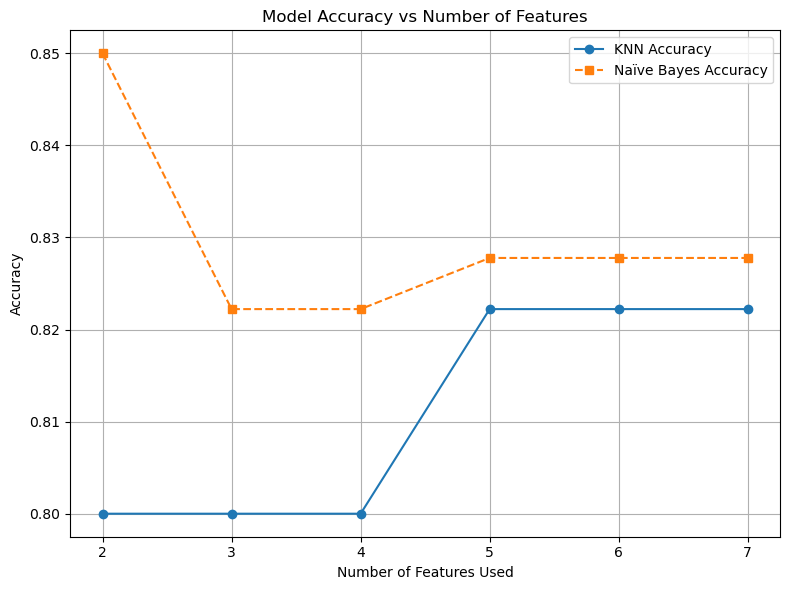
\includegraphics[width=0.6\textwidth]{figures/feature_accuracy_comparison.png}
    \caption{Accuracy progression across increasing features (Raisin)}
    \label{fig:feature_progression}
\end{figure}

Figure~\ref{fig:feature_progression} shows that Naïve Bayes performed better with fewer features, but plateaued quickly. KNN, on the other hand, benefited from more features and offered stable performance.

\section{Confusion Matrix Analysis}
\label{sec:comp_confmat}

Confusion matrices reveal deeper insights into the models’ prediction behavior. Table~\ref{tab:htru2_knn_cm} shows the confusion matrix for HTRU2 using KNN.

\begin{table}[H]
    \centering
    \caption{KNN Confusion Matrix (HTRU2, 98.27\% Accuracy)}
    \label{tab:htru2_knn_cm}
    \begin{tabular}{|c|c|c|}
        \hline
        & \textbf{Predicted 0} & \textbf{Predicted 1} \\
        \hline
        \textbf{Actual 0} & 3242 & 17 \\
        \textbf{Actual 1} & 45 & 276 \\
        \hline
    \end{tabular}
\end{table}

The low false positive and false negative values for KNN on HTRU2 emphasize its superior classification boundary.

\section{Model Behavior Summary}
\label{sec:comp_summary}

\begin{itemize}
    \item \textbf{KNN} consistently performed well with increasing features, especially for high-dimensional datasets like HTRU2.
    \item \textbf{Naïve Bayes} peaked early in the Raisin dataset due to strong assumptions about feature independence and smaller data size.
    \item For large datasets with continuous features and subtle class separations, \textbf{KNN is the recommended model}.
\end{itemize}

\section{Visual Summary}

\begin{figure}[H]
    \centering
    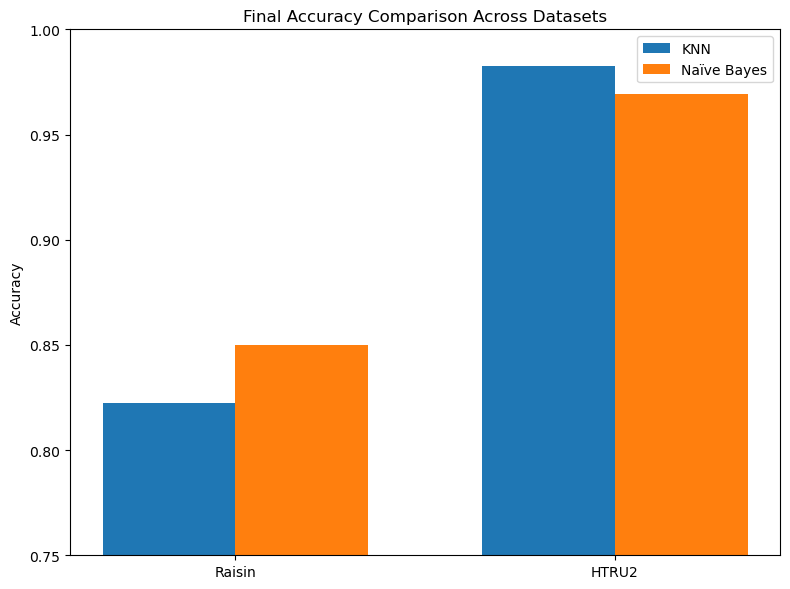
\includegraphics[width=0.6\textwidth]{figures/final_model_comparison.png}
    \caption{Overall Accuracy Comparison Between Models and Datasets}
    \label{fig:final_model_chart}
\end{figure}

Figure~\ref{fig:final_model_chart} summarizes the accuracy across both datasets and models in a single view.

\section{Conclusion}

The experiments confirmed that model performance is highly dependent on dataset characteristics. While Naïve Bayes is computationally efficient, KNN’s ability to leverage feature geometry made it more accurate and adaptable in most scenarios.
